%
% This document contains the chapter about synthesizing circuits.
%
% Copyright (C) 2005, 2006 Stefan Jahn <stefan@lkcc.org>
% Copyright (C) 2005 Michael Margraf <Michael.Margraf@alumni.TU-Berlin.DE>
%
% Impedance matching documentation:
% Copyright (C) 2017 Andres Martínez-Mera <andresmartinezmera@gmail.com>
%
% Permission is granted to copy, distribute and/or modify this document
% under the terms of the GNU Free Documentation License, Version 1.1
% or any later version published by the Free Software Foundation.
%

\chapter{Synthesizing circuits}
\label{sec:synthesis}

\section{Attenuators}

Attenuators are used to damp a signal. Using pure ohmic resistors
the circuit can be realized for a very high bandwidth, i.e. from
DC to many GHz. The power attenuation $0 < L\le 1$ is defined as:
\begin{equation}
\label{eqn:loss}
L = \dfrac{P_{in}}{P_{out}}
  = \dfrac{V_{in}^2}{Z_{in}}\cdot\dfrac{Z_{out}}{V_{out}^2}
  = \left( \dfrac{V_{in}}{V_{out}}\right)^2 \cdot\dfrac{Z_{out}}{Z_{in}}
\end{equation}
where $P_{in}$ and $P_{out}$ are the input and output power and
$V_{in}$ and $V_{out}$ are the input and output voltages.

\begin{figure}[ht]
\begin{center}
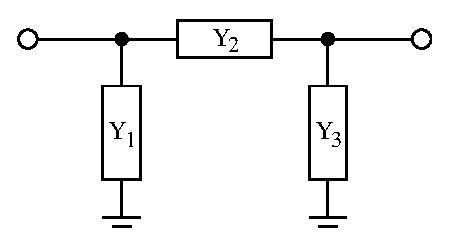
\includegraphics[width=5cm]{picircuit}
\end{center}
\caption{$\pi$-topology of an attenuator}
\label{fig:pi_attenuator}
\end{figure}
\FloatBarrier

Fig. \ref{fig:pi_attenuator} shows an attenuator using the
$\pi$-topology. The conductances can be calculated as follows.
\begin{align}
Y_2 & = \dfrac{L - 1}{2\cdot \sqrt{L\cdot Z_{in}\cdot Z_{out}}} \\
Y_1 & = Y_2\cdot\left( \sqrt{\dfrac{Z_{out}}{Z_{in}}\cdot L} - 1 \right) \\
Y_3 & = Y_2\cdot\left( \sqrt{\dfrac{Z_{in}}{Z_{out}}\cdot L} - 1 \right)
\end{align}
where $Z_{in}$ and $Z_{out}$ are the input and output reference
impedances, respectively. The $\pi$-attenuator can be used for an
impedance ratio of:
\begin{equation}
\dfrac{1}{L} \le \dfrac{Z_{out}}{Z_{in}} \le L
\end{equation}

\begin{figure}[ht]
\begin{center}
\includegraphics[width=5cm]{tcircuit}
\end{center}
\caption{T-topology of an attenuator}
\label{fig:t_attenuator}
\end{figure}
\FloatBarrier

Fig. \ref{fig:t_attenuator} shows an attenuator using the
T-topology. The resistances can be calculated as follows.
\begin{align}
Z_2 & = \dfrac{2\cdot \sqrt{L\cdot Z_{in}\cdot Z_{out}}}{L - 1} \\
Z_1 & = Z_{in}\cdot A - Z_2 \\
Z_3 & = Z_{out}\cdot A - Z_2 \\
\textrm{with} \qquad A & = \dfrac{L + 1}{L - 1}
\end{align}
where $L$ is the attenuation ($0 < L\le 1$) according to
equation \ref{eqn:loss} and $Z_{in}$ and $Z_{out}$
are the input and output reference impedance, respectively.
The T-attenuator can be used for an impedance ratio of:
\begin{equation}
\dfrac{Z_{out}}{Z_{in}} \le \dfrac{(L+1)^2}{4\cdot L}
\end{equation}

\section{Filters}

One of the most common tasks in microwave technologies is to
extract a frequency band from others. Optimized filters exist
in order to easily create a filter with an appropriate characteristic.
The most popular ones are:

\addvspace{12pt}

\begin{tabular}{l|l}
Name & Property \\
\hline
Bessel filter (Thomson filter) & as constant group delay as possible \\
Butterworth filter (power-term filter) & as constant amplitude transfer function as possible \\
Chebychev filter type I & constant ripple in pass band \\
Chebychev filter type II & constant ripple in stop band \\
Cauer filter (elliptical filter) & constant ripple in pass and stop band \\
\end{tabular}

\addvspace{12pt}

From top to bottom the following properties increase:
\begin{itemize}
\item ringing of step response
\item phase distortion
\item steepness of amplitude transfer function at the beginning of the pass band
\end{itemize}

\addvspace{12pt}

The order $n$ of a filter denotes the number of poles of its (voltage)
transfer function. It is:
\begin{equation}
\text{slope of asymptote} = \pm\, n\cdot 20 \text{dB/decade}
\end{equation}
Note that this equation holds for all filter characteristics, but
there are big differences concerning the attenuation near the pass
band.


\subsection{LC ladder filters}

The best possibility to realize a filters in VHF and UHF bands are
LC ladder filters. The usual way to synthesize them is to first
calculate a low-pass (LP) filter and afterwards transform it into a
high-pass (HP), band-pass (BP) or band-stop (BS) filter. To do so,
each component must be transformed into another.

\addvspace{12pt}

In a low-pass filter, there are  parallel capacitors $C_{LP}$ and
series inductors $L_{LP}$ in alternating order. The other filter
classes can be derived from it:

\addvspace{12pt}

In a high-pass filter:
\begin{align}
C_{LP} \quad \rightarrow \quad & L_{HP} = \dfrac{1}{\omega_B^2\cdot C_{LP}} \\
L_{LP} \quad \rightarrow \quad & C_{HP} = \dfrac{1}{\omega_B^2\cdot L_{LP}}
\end{align}

\addvspace{12pt}

In a band-pass filter:
\begin{align}
C_{LP} \quad \rightarrow \quad & \text{parallel resonance circuit with} \\
                               & C_{BP} = \dfrac{C_{LP}}{\Delta\Omega} \\
                               & L_{BP} = \dfrac{\Delta\Omega}{\omega_1\cdot \omega_2\cdot C_{LP}} \\
L_{LP} \quad \rightarrow \quad & \text{series resonance circuit with} \\
                               & C_{BP} = \dfrac{\Delta\Omega}{\omega_1\cdot \omega_2\cdot L_{LP}} \\
                               & L_{BP} = \dfrac{L_{LP}}{\Delta\Omega}
\end{align}

\addvspace{12pt}

In a band-stop filter:
\begin{align}
C_{LP} \quad \rightarrow \quad & \text{series resonance circuit with} \\
       & C_{BP} = \dfrac{C_{LP}}{2\cdot\left| \dfrac{\omega_2}{\omega_1} - \dfrac{\omega_1}{\omega_2} \right| } \\
       & L_{BP} = \dfrac{1}{\omega^2\cdot \Delta\Omega\cdot C_{LP}} \\
L_{LP} \quad \rightarrow \quad & \text{parallel resonance circuit with} \\
       & C_{BP} = \dfrac{1}{\omega^2\cdot \Delta\Omega\cdot L_{LP}} \\
       & L_{BP} = \dfrac{L_{LP}}{2\cdot\left| \dfrac{\omega_2}{\omega_1} - \dfrac{\omega_1}{\omega_2} \right| }
\end{align}

\addvspace{12pt}

Where
\begin{align}
\omega_1 \quad\rightarrow\quad & \text{lower corner frequency of frequency band} \\
\omega_2 \quad\rightarrow\quad & \text{upper corner frequency of frequency band} \\
\omega   \quad\rightarrow\quad & \text{center frequency of frequency band} \quad \omega = 0.5\cdot (\omega_1 + \omega_2) \\
\Delta\Omega \quad\rightarrow\quad & \Delta\Omega = \dfrac{|\omega_2 - \omega_1|}{\omega}
\end{align}

\subsubsection{Butterworth}

The $k$-th element of an $n$ order Butterworth low-pass ladder filter is:
\begin{alignat}{3}
 & \text{capacitance:} \qquad & C_k = & \dfrac{X_k}{Z_0} \\
 & \text{inductance:}  \qquad & L_k = & X_k \cdot Z_0 \\
 & \text{with}         \qquad & X_k = & \dfrac{2}{\omega_B} \cdot \sin \dfrac{(2\cdot k + 1)\cdot\pi}{2\cdot n}
\end{alignat}

The order of the Butterworth filter is dependent on the specifications
provided by the user.  These specifications include the edge
frequencies and gains.
\begin{equation}
\label{eq:ButtOrder}
n = \dfrac{\log{\left(\dfrac{10^{-0.1\cdot \alpha_{stop}} - 1}{10^{-0.1\cdot \alpha_{pass}} - 1}\right)}}{2\cdot\log{\left(\dfrac{\omega_{stop}}{\omega_{pass}}\right)}}
\end{equation}

\subsubsection{Chebyshev I}

The equations for a Chebyshev type I filter are defined recursivly.
With $R_{dB}$ being the passband ripple in decibel, the $k$-th
element of an $n$ order low-pass ladder filter is:
\begin{alignat}{3}
 & \text{capacitance:} \qquad & C_k & = \dfrac{X_k}{Z_0} \\
 & \text{inductance:}  \qquad & L_k & = X_k \cdot Z_0 \\
 & \text{with}         \qquad & X_k & = \dfrac{2}{\omega_B}\cdot g_k \\
 & & r   & = \sinh\left( \frac{1}{n}\cdot\text{arsinh}\dfrac{1}{\sqrt{10^{R_{dB}/10} - 1}} \right) \\
 & & a_k & = \sin \dfrac{(2\cdot k + 1)\cdot\pi}{2\cdot n} \\
 & & g_k & =
\begin{cases}
\begin{array}{ll}
  \dfrac{a_k}{r} & \textrm{ for } \quad k=0\\
  \dfrac{a_{k-1}\cdot a_k}{g_{k-1}\cdot \left( r^2 + \sin^2\dfrac{k\cdot\pi}{n} \right)} & \textrm{ for } \quad k\ge 1
\end{array}
\end{cases} \\
 & & X_k & = \dfrac{2}{\omega_B}\cdot g_k
\end{alignat}

The order of the Chebychev filter is dependent on the specifications
provided by the user.  The general form of the calculation for the
order is the same as for the Butterworth, except that the inverse
hyperbolic cosine function is used in place of the common logarithm
function.
\begin{equation}
\label{eq:ChebOrder}
n = \dfrac{\textrm{sech}\left(\dfrac{10^{-0.1\cdot \alpha_{stop}} - 1}{10^{-0.1\cdot \alpha_{pass}} - 1}\right)}{2\cdot\textrm{sech}\left(\dfrac{\omega_{stop}}{\omega_{pass}}\right)}
\end{equation}

\subsubsection{Chebyshev II}

Because of the nature of the derivation of the inverse Chebychev approximation function from the standard Chebychev approximation the calculation of the order \eqref{eq:ChebOrder} is the same.

\subsection{Quarter wavelength filters}

Quarter wavelength filters are based on the fact that short and open $\lambda/4$ stubs are equivalent to series and paralell resonant tanks, respectively. Once given the normalized $g_i$ coefficients of the filter prototype, it is quite straighforward to obtain the impedance of the short/open stubs, depending on the desired filter mask (bandpass/notch). Figure \ref{eq:QWfilter} illustrates the topology of a quarter wavelength filter.\\

\begin{figure}[h!]
\centering
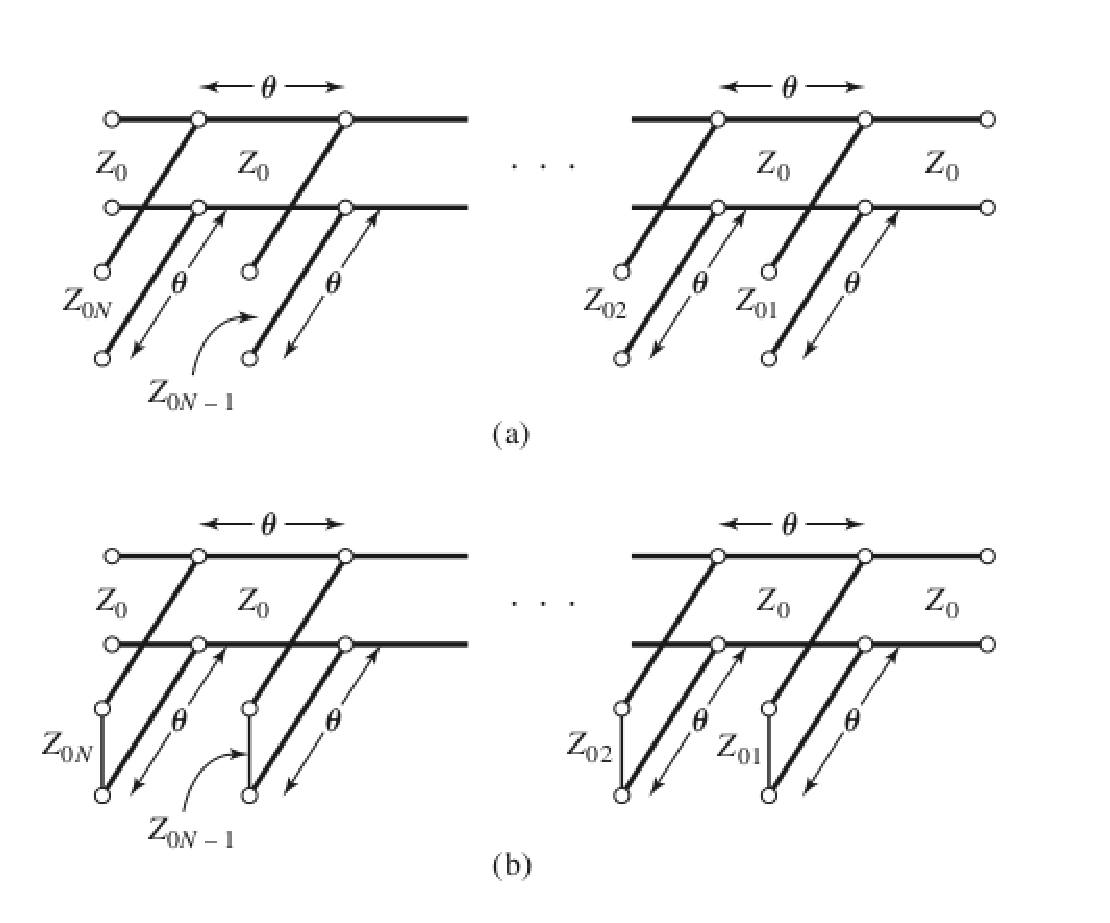
\includegraphics[width=100mm]{QuarterWavelengthFilter}
\caption{Quarter wavelength filters topology. a) Notch filter b) Bandpass filter \cite{Pozar}}
\label{eq:QWfilter}
\end{figure}

\noindent The impedance of the $i$-th stub, $Z_i$, is given by:

\begin{itemize}
\item{Bandpass (short circuit)} $Z_i = \frac{\pi Z_0 \Delta}{4g_i}$
\item{Notch (open circuit)} $Z_i = \frac{4 Z_0 }{g_i\pi \Delta}$
\end{itemize}

\noindent where $Z_0$ is the characteristic impedance of the filter (typically, 50$\Omega$) and $\Delta$ is the relative bandwidth defined as $\Delta = \frac{f_2 - f_1}{f_c}$. The demonstration \cite{Pozar} is not included in this document in favour of greater simplicity.

\noindent It has to be said that quarter wavelength filters are narrowband by nature. Besides this, these kind of filters may not be feasible because of the stubs may require unpractical widths (i.e. impedances) for proper operation.


\section{Matching newtworks}
The purpose of a matching network is to transform an impedance into another (e.g. convert the impedance of a device to the characteristic impedance of a transmission line, $Z_0$) and play an important role in RF circuit design. The matching networks can be implemented with lumped components (typically in applications below $<$ 1GHz), but also with transmission lines (more common in the microwave band). The following sections show the basics of the most common matching network synthesis techniques as well as the design equations implemented in the Qucs impedance matching tool.

\subsection{L-section}
The \textit{L-section} method combines two reactances (shunt and series) to match any complex load impedance, $Z_L = R_L + jX_L$ to a source impedance, $Z_0$, (typically, $Z_0 = 50\Omega$) at a certain frequency. As shown in \ref{fig:Lsection}, eight different combinations of inductor and capacitor can be used depending on where $Z_L$ is located on the Smith chart.

\begin{figure}[H]
\centering
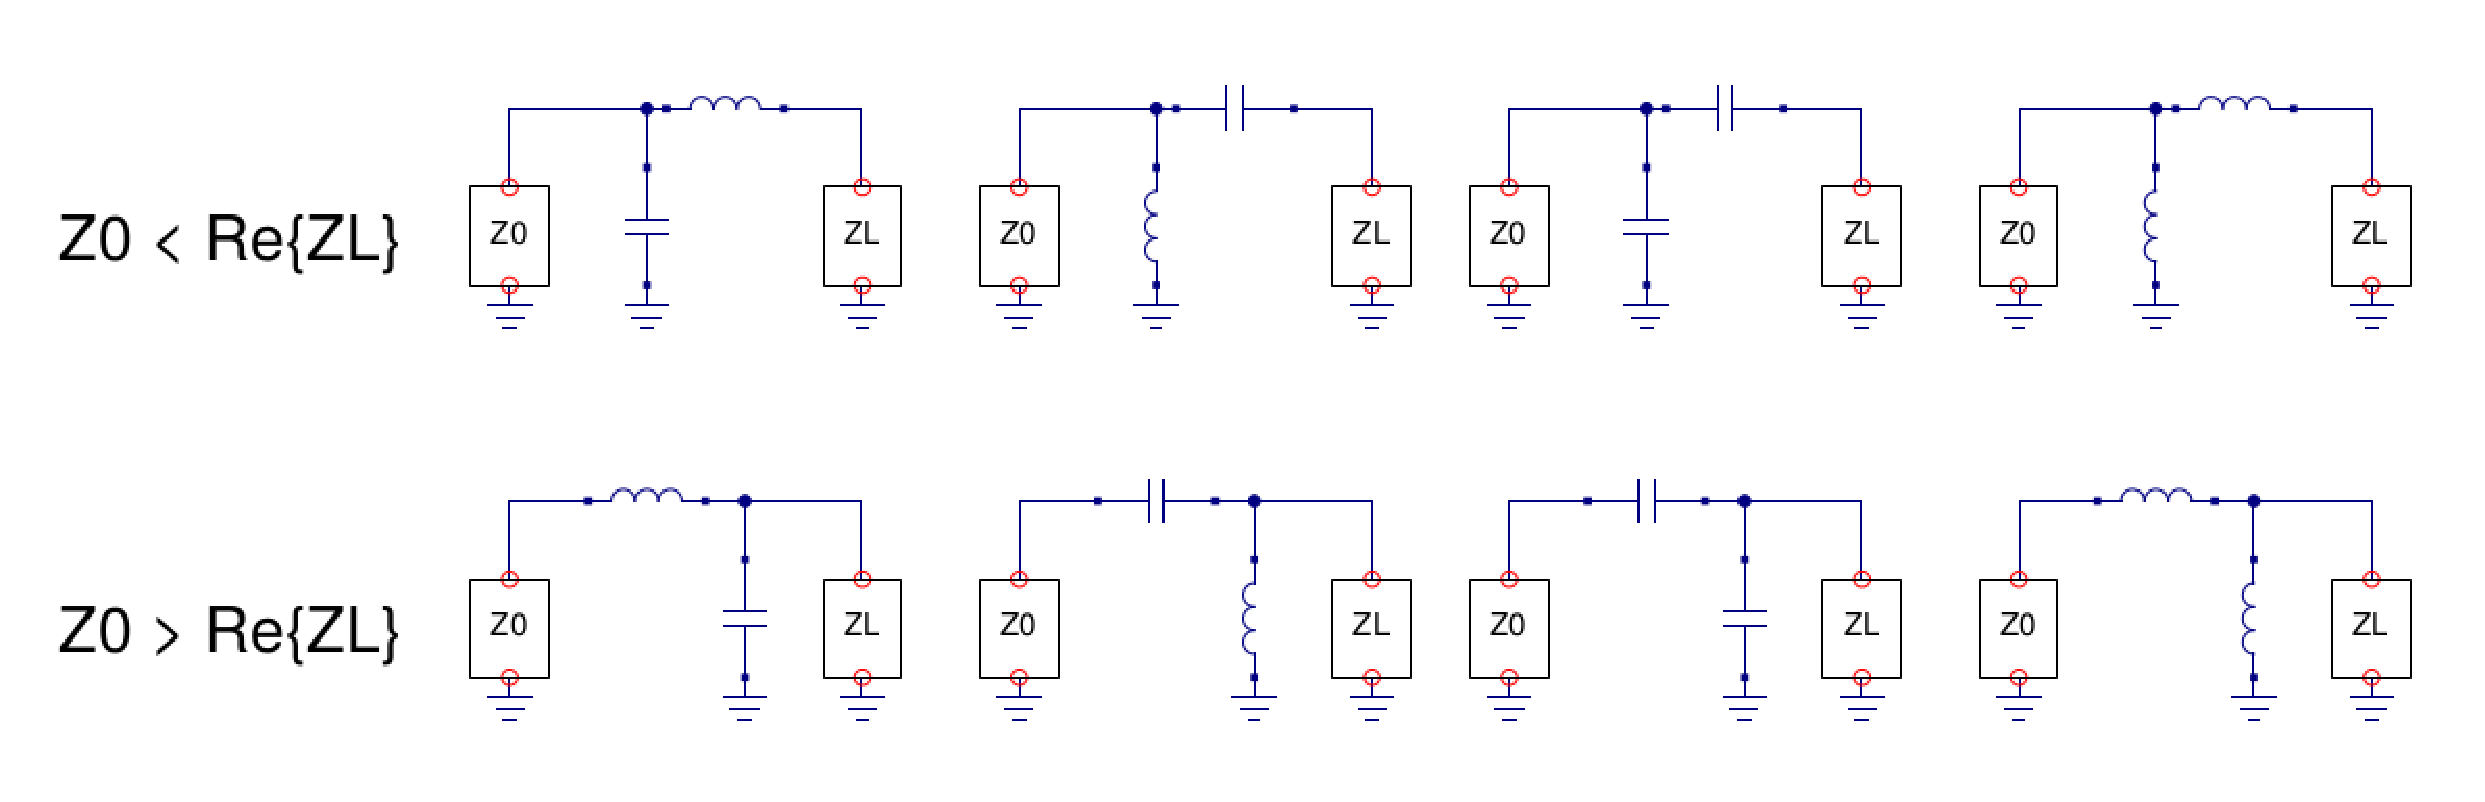
\includegraphics[width=120mm]{Lsection}
\caption{L-section topology}
\label{fig:Lsection}
\end{figure}

The series and the shunt reactances move $Z_L$ towards $Z_0$ through the impedance and admittance circles respectively. As shown at \ref{fig:LsectionSmith}, these eight combinations of series and shunt reactances provide the required degrees of freedom to move $Z_L$ to any other point in the Smith chart.


\begin{figure}[H]
\centering
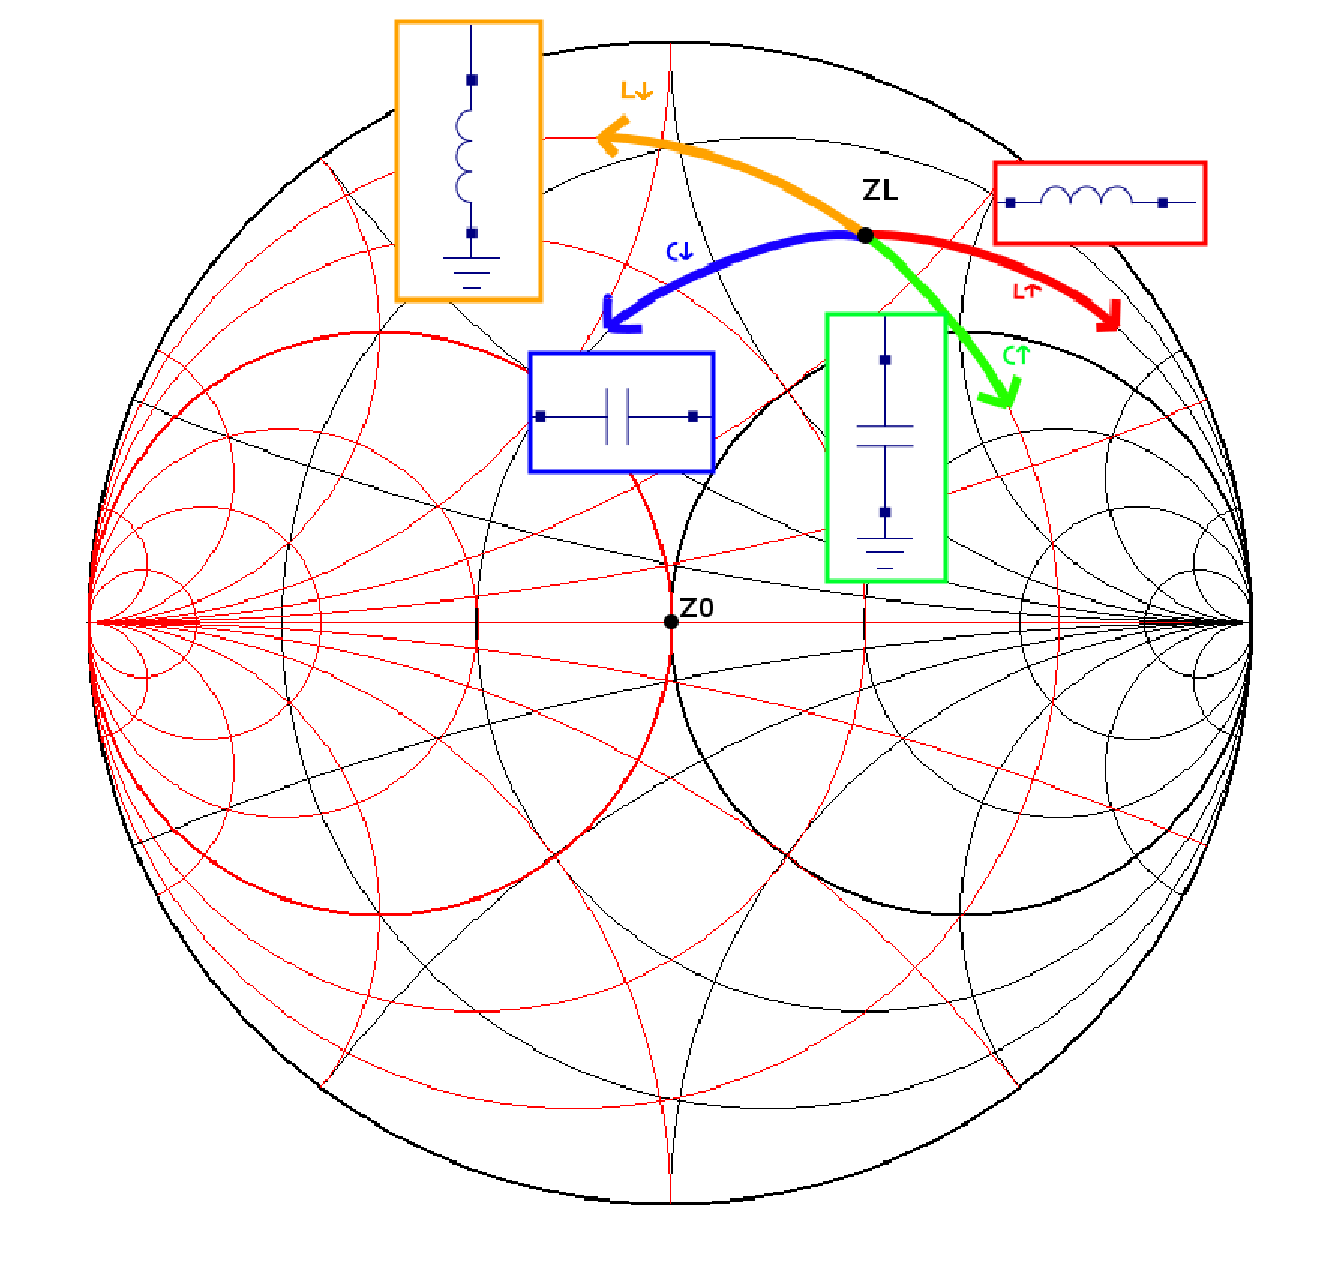
\includegraphics[width=120mm]{SmithChart-Lsection}
\caption{Impedance traslation produced by a series/shunt capacitor and inductor}
\label{fig:LsectionSmith}
\end{figure}


\noindent The design equations for the \textit{L-section} method are the following:\\

if $\frac{R_L}{Z_0} > 1$

\begin{align}
B & = \frac{X_L \pm \sqrt{\frac{R_L}{Z_0}} \cdot \sqrt{R_L^2 + X_L^2 - Z_0\cdot R_L}}{R_L^2 + X_L^2} \\
X & = \frac{1}{B} + \frac{X_L \cdot Z_0}{R_L} - \frac{Z_0}{B \cdot R_L}
\end{align}

\noindent on the counterpart, if $\frac{R_L}{Z_0} < 1$

\begin{align}
X & = \pm \sqrt{R_L \cdot (Z_0 - R_L)} - X_L \\
B & = \pm \frac{(Z_0 - R_L)/R_L}{Z_0}
\end{align}


\noindent \textit{Reference:} \cite{Pozar}, pages 229-233.

\subsection{Single stub}

At microwave frequencies, transmission lines are usually preferred rather than lumped components. The simplest method to achieve narrowband matching with transmission lines is to use a stub and a transmission line.

\begin{table}[H]
  \centering
  \begin{tabular}{ | c | c | }
    \hline
    Open circuited stub & Short circuited stub\\ \hline
    \begin{minipage}{.4\textwidth}
      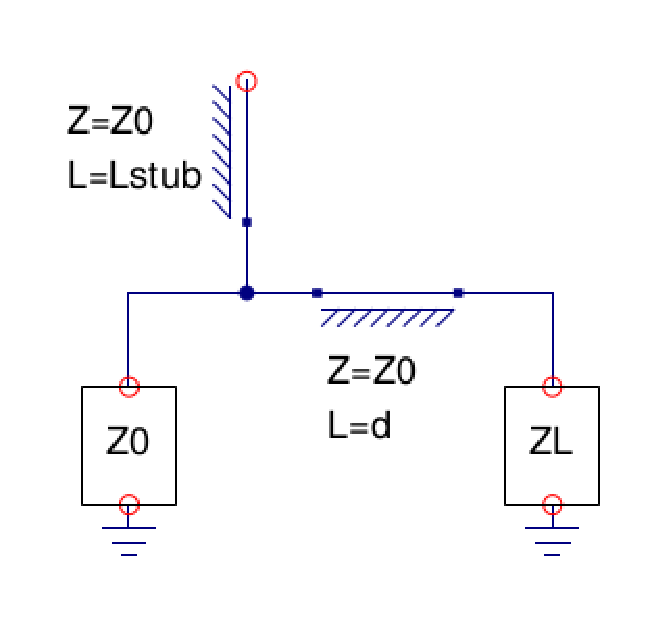
\includegraphics[width=\linewidth]{SingleStubOpen}
    \end{minipage}
    &
    \begin{minipage}{.4\textwidth}
      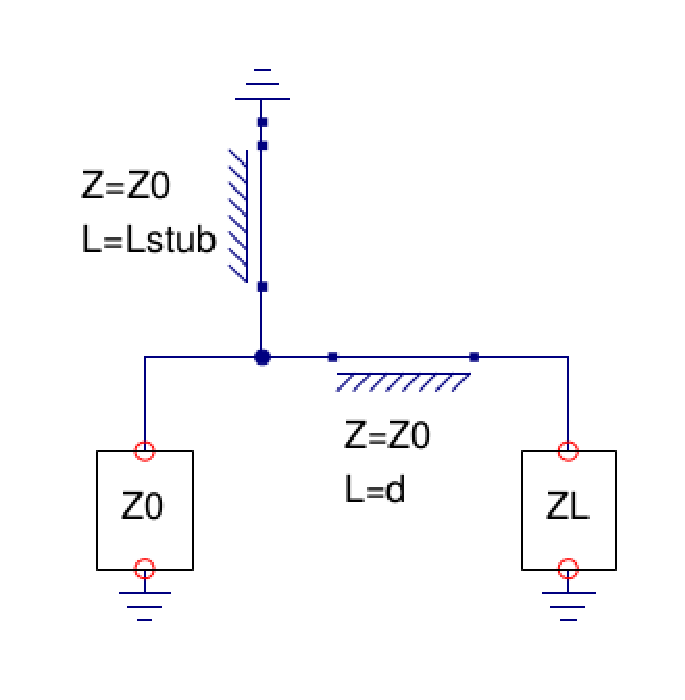
\includegraphics[width=\linewidth]{SingleStubShort}
    \end{minipage}
    \\ \hline
  \end{tabular}
  \caption{Single stub matching}
  \label{tbl:sngstub}
\end{table}


As \ref{fig:SmithTL} shows, a transmission line describes a circle around $Z_0$ whereas an open and a short circuited stub behave like a shunt capacitor and a shunt inductor respectively, which gives the necessary degrees of freedom to match any complex load, $Z_L$ to $Z_0$:

\begin{figure}[H]
\centering
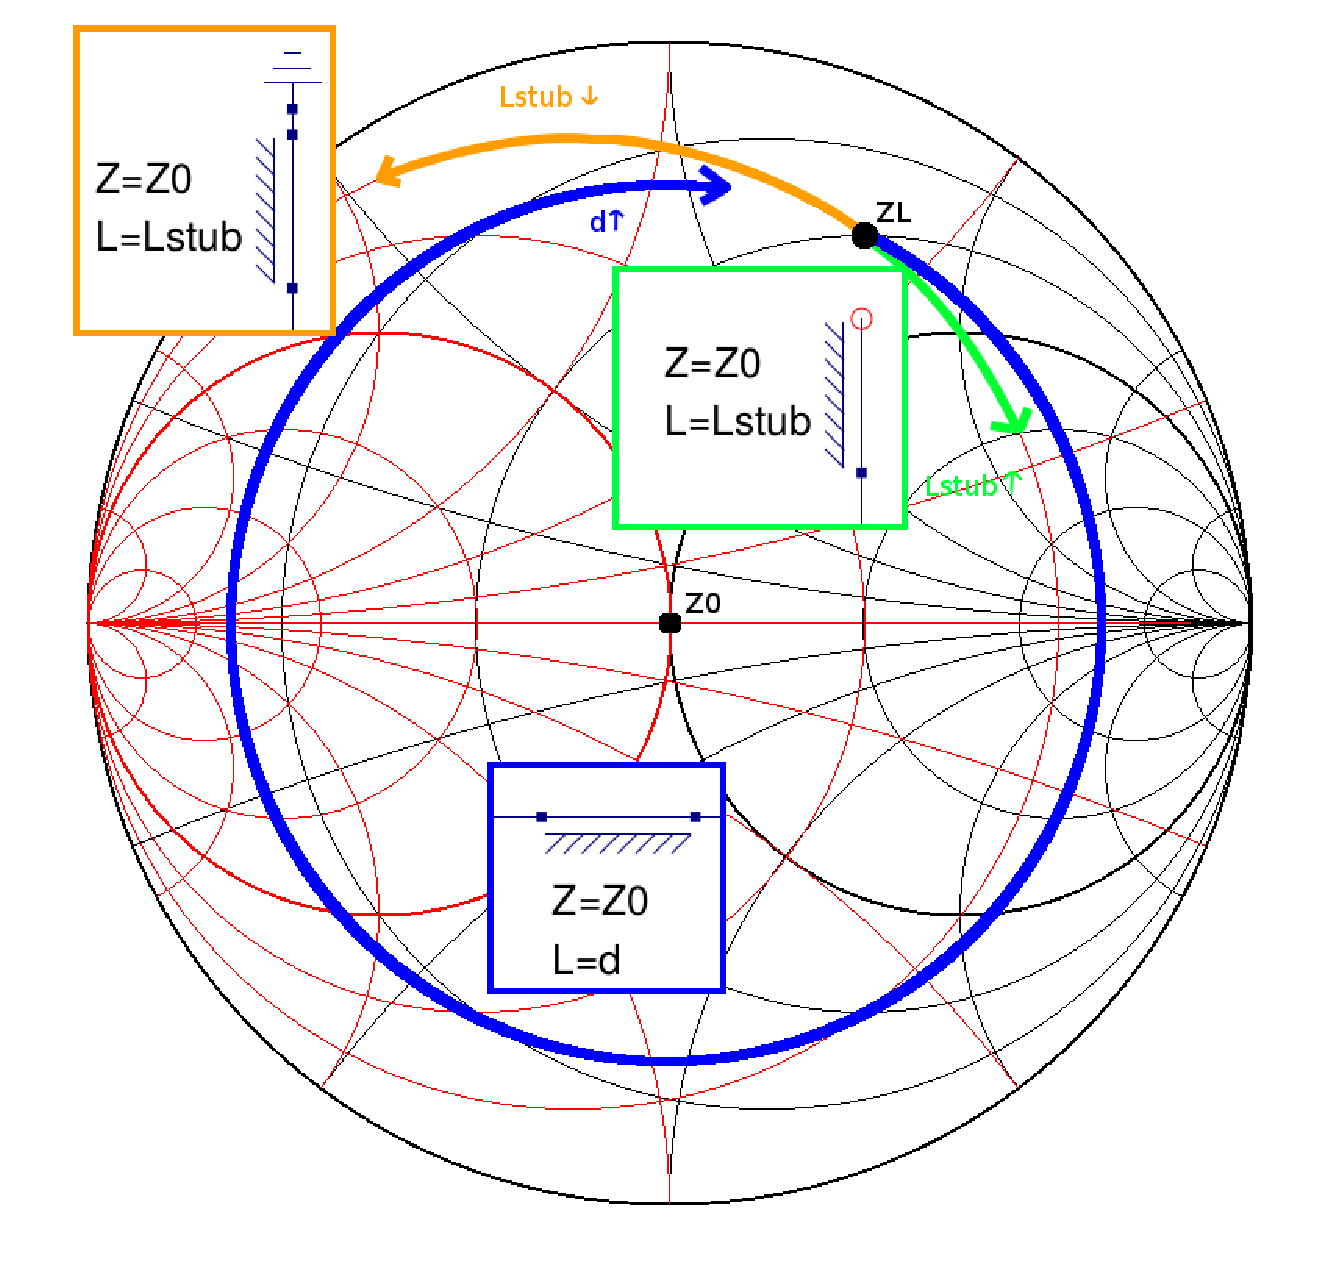
\includegraphics[width=120mm]{SmithChartTL}
\caption{Impedance traslation caused by a transmission line and an open/short circuited stub}
\label{fig:SmithTL}
\end{figure}


\noindent Below are detailed the design equations for the \textit{single stub} technique, where the variables are the distance between the stub and the load, and the length of the stub. The impedance seen at the stub, $Z(d)$ is given by:

\begin{equation}
Z(d) = Z_0 \frac{Z_L + j\cdot Z_0\cdot tan(\beta \cdot d)}{Z_0 + j\cdot Z_L \cdot tan(\beta \cdot d)}
\end{equation}

\noindent where $\beta = \frac{2\pi}{\lambda}$ is the wave number and $d$ the distance between the load and the stub. The admittance at the stub is: $Y(d) = G(d)+j \cdot B(d)$, where G(d) is the conductance and B(d) the susceptance at d. It can be shown that:

\begin{equation}
G(d) = \frac{R_L \cdot (1 + tan^2(\beta \cdot d))}{R_L^2 + (X_L + Z_0\cdot tan(\beta \dot d))^2}
\end{equation}

\noindent and,

\begin{equation}
B(d) = \frac{R_L^2\cdot tan(\beta \cdot d) - (Z_0 - X_L\cdot tan(\beta \cdot d))\cdot (X_L + Z_0\cdot tan(\beta \cdot d))}{Z_0 \cdot (R_L^2 + (X_L + Z_0\cdot tan(\beta \cdot d))^2)}
\end{equation}

The conductance at the stub should be $G(d) = 1/Z_0$ so as to match the real part of the load to $Z_0$. Then, applying this condition and solving the previous equation for $t = tan(\beta \cdot d)$, it gives:

\begin{align}
R_L \neq Z_0 \;\;\;\;\;\;\;  t & = \frac{X_L \pm \sqrt{(R_L/Z_0) \cdot ((Z_0 - R_L)^2 + X_L^2)}}{R_L - Z_0} \\
R_L == Z_0 \;\;\;\;\;\;\;  t & = -X_L/(2\cdot Z_0)
\end{align}

\noindent Now, the susceptance of the stub should be calculated to cancel the reactive part of the load impedance, so $B_{stub} = -B(d)$.

\noindent Since $t=tan(\beta \cdot d)$, $d$ can be calculated as:

\begin{align}
\text{if t $\geq$ 0}\;\;\;\;\;\;\;  d & = \frac{\lambda}{2\pi} atan(t) \\
\text{if t $<$ 0}\;\;\;\;\;\;\;  d & = \frac{\lambda}{2\pi} (\pi + atan(t))
\end{align}

\noindent The length of the stub is given by:

\begin{align}
\text{Open circuited stub} \;\;\;\;\;\;\;  l_{open} & = \frac{-\lambda}{2\pi} atan\left(Z_0\cdot B(d)\right)  \\
\text{Short circuited stub}\;\;\;\;\;\;\;  l_{short} & = \frac{\lambda}{2\pi} atan\left(\frac{1}{Z_0\cdot B(d)}\right)
\end{align}

\noindent Finally, if needed, the stubs may be splitted into balanced stubs as follows:

\begin{table}[H]
  \centering
  \begin{tabular}{ | c | c | }
    \hline
    Open circuited balanced stubs & Short circuited balanced stubs\\ \hline
    \begin{minipage}{.4\textwidth}
      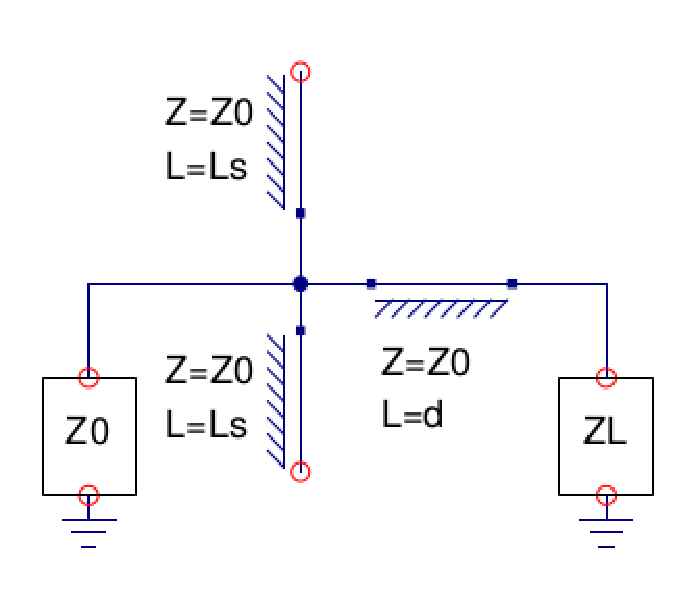
\includegraphics[width=\linewidth]{SingleStubOpenBalanced}
    \end{minipage}
    &
    \begin{minipage}{.4\textwidth}
      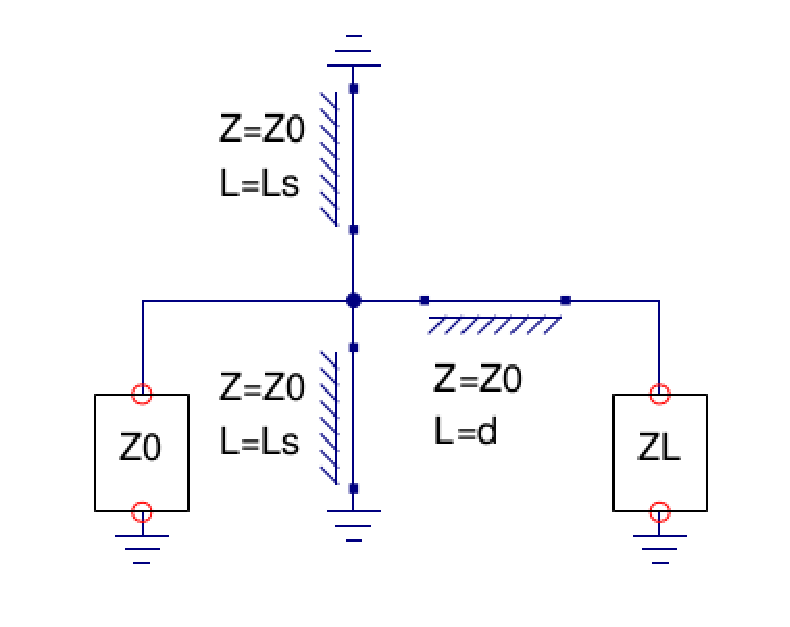
\includegraphics[width=\linewidth]{SingleStubShortBalanced}
    \end{minipage}
    \\ \hline
  \end{tabular}
  \caption{Single stub matching (balanced stubs)}\label{tbl:sngstubbalanced}
\end{table}

\noindent The length of the balanced stubs is given by the following equations \cite{SanDiegoNotesMatching}:

\begin{align}
\text{Open circuited stub:} \;\;\;\;\;\;\; l_{sb} & = \frac{\lambda}{2\pi} tan^{-1} \left( 2 tan\left( \frac{2\pi l_s}{\lambda}\right)\right) \\
\text{Short circuited stub:}\;\;\;\;\;\;\; l_{sb} & = \frac{\lambda}{2\pi} tan^{-1} \left( \frac{1}{2} tan\left( \frac{2\pi l_s}{\lambda}\right)\right)
\end{align}

where $l_{sb}$ and $l_{s}$ are the lengths of the unbalanced and balanced stubs respectively.\\

\noindent \textit{Reference:} \cite{Pozar}, pages 234-241.


\subsection{Double stub}
The distance between different blocks (e.g. amplifier stages, filters,...) in a board is determined by the transmission line, so the its length is not easily tunable in practice. Obviously, this fact locks one degree of freedom in the \textit{single stub} technique, making it less suitable. On the counterpart, the \textit{double stub} method keeps the length of the transmission line fixed, so tuning can be done simply by adjusting the length of the stubs. This is usually far more convenient since the stubs can be trimmered or elongated as needed. However, this technique comes with the disadvantage of having restrictions about the load to be matched, $Z_L$.

\begin{table}[H]
  \centering
  \begin{tabular}{ | c | c | }
    \hline
    Open circuited stub & Short circuited stub\\ \hline
    \begin{minipage}{.4\textwidth}
      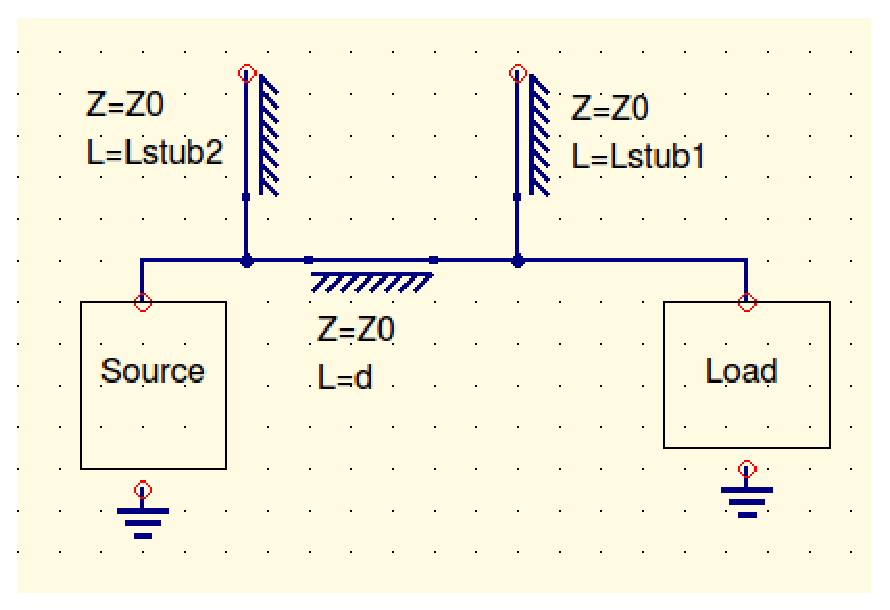
\includegraphics[width=\linewidth]{DoubleStubOpen}
    \end{minipage}
    &
    \begin{minipage}{.4\textwidth}
      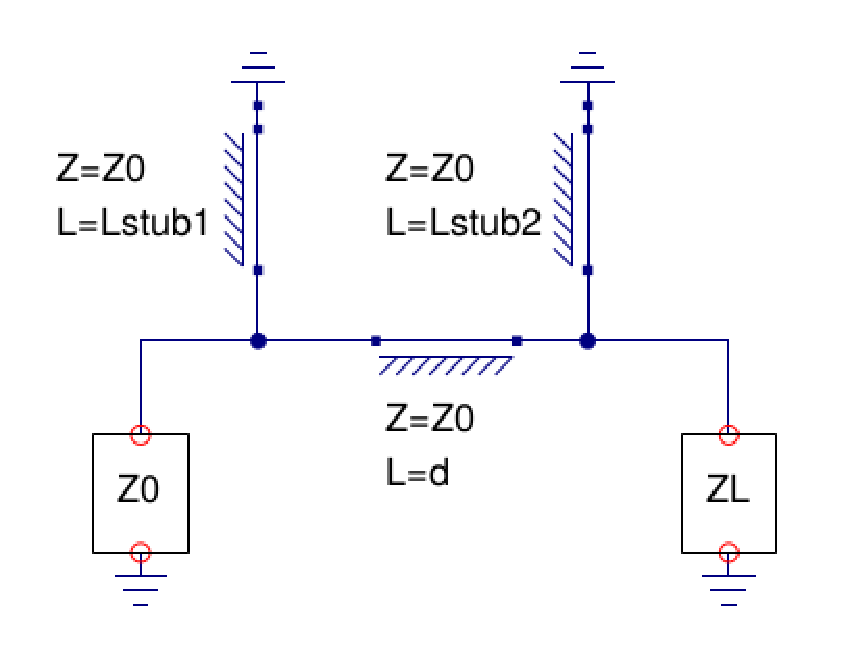
\includegraphics[width=\linewidth]{DoubleStubShort}
    \end{minipage}
    \\ \hline
  \end{tabular}
  \caption{Double stub matching}\label{tbl:dblstub}
\end{table}


The admittance at the first stub is $Y_1 = G_L + j(B_L + B_{stub_1})$, where $Y_L$, $B_L$ and $G_L$ have the same meaning as in the previous section. $B_{stub1}$ is the susceptance of the first stub.

The distance between the stubs, $d$, is typically fixed to $\lambda/8$. Under this condition, the admittance at the second stub is given by:

\begin{equation}
Y_2 = Y_0 \frac{G_L + j(B_L + B_{stub1} + Y_0 \cdot tan(\beta \cdot d))}{Y_0 + j (G_L + j(B_L + B_{stub1})) \cdot tan(\beta \cdot d)}
\end{equation}

\noindent The impedance at the second stub must be $Z_0$, so equating $Real\lbrace Y_2 \rbrace = 1/Z_0$ it gives:

\begin{equation}
G_L = Y_0\frac{1 + tan^2(\beta \cdot d)}{2tan^2(\beta \cdot d)} \lbrace 1 \pm \sqrt{1 - \frac{4tan^2(\beta \cdot d)(Y_0 - (B_L+B_{stub1})\cdot tan(\beta \cdot d))^2}{Y_0^2(1+tan^2(\beta \cdot d))^2}} \rbrace
\end{equation}

Notice here that those conductances which make the factor inside the square root negative cannot be matched. So, the \textit{double stub} method is limited to load conductances which meet the following condition:

\begin{equation}
G_L \leq \frac{Y_0}{sin^2(\beta \cdot d)}
\end{equation}

\noindent The susceptance of the first stub can be calculated as:
\begin{equation}
B_{stub_1} = - B_L + \frac{Y_0 \pm \sqrt{(1 + tan^2(\beta \cdot d))G_L\cdot Y_0 - (G_L \cdot tan(\beta \cdot d))^2}}{tan(\beta \cdot d)}
\end{equation}


\noindent Similarly, the susceptance of the second stub is:
\begin{equation}
B_{stub_2} = \frac{\pm\sqrt{Y_0\cdot G_L(1 + tan^2(\beta \cdot d)) - (G_L\cdot tan(\beta \cdot d))^2} + G_L \cdot Y_0}{G_L \cdot tan(\beta \cdot d)}
\end{equation}

\noindent Finally, the length of the stubs is given by:

\begin{align}
l_{open} & = \frac{\lambda}{2\pi} atan\left(Z_0\cdot B_{stub_i}\right)   & \text{Open stub}\\
l_{short} & = \frac{-\lambda}{2\pi} atan\left(\frac{1}{Z_0\cdot B_{stub_i}}\right) & \text{Short circuited stub}
\end{align}

\noindent where $i=\lbrace 1,2 \rbrace$ denotes the number of the stub.\\

\noindent As in \textit{single stub} method, the use of balanced stubs is possible:

\begin{table}[H]
  \centering
  \begin{tabular}{ | c | c | }
    \hline
    Open circuited stub & Short circuited stub\\ \hline
    \begin{minipage}{.4\textwidth}
      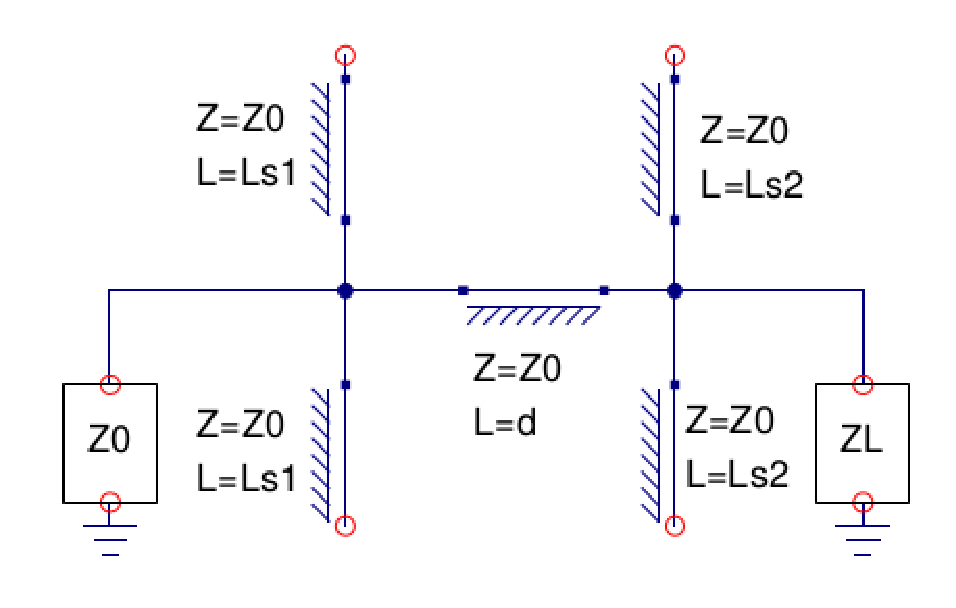
\includegraphics[width=\linewidth]{DoubleStubOpenBalanced}
    \end{minipage}
    &
    \begin{minipage}{.4\textwidth}
      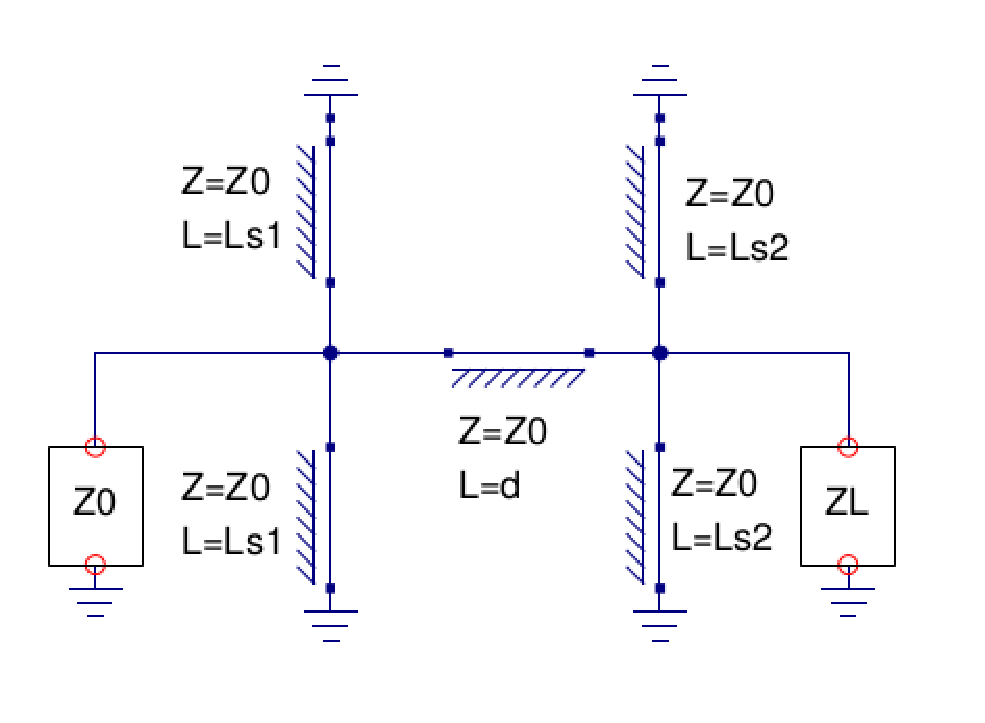
\includegraphics[width=\linewidth]{DoubleStubShortBalanced}
    \end{minipage}
    \\ \hline
  \end{tabular}
  \caption{Double stub matching (balanced stubs)}\label{tbl:dblstubbalanced}
\end{table}

\noindent \textit{Reference} \cite{Pozar}, pages 241-246.

\subsection{$\lambda/4 + \lambda/8$ matching}
Another narrowband matching network technique is to combine a $\lambda/4$ and $\lambda/8$ transmission to match a complex impedance, $Z_L$ to real source impedance. The $\lambda/8$ line converts the complex impedance to a real one and the $\lambda/4$ line converts that intermediate real impedance into the source impedance, $Z_0$.

\begin{figure}[H]
\centering
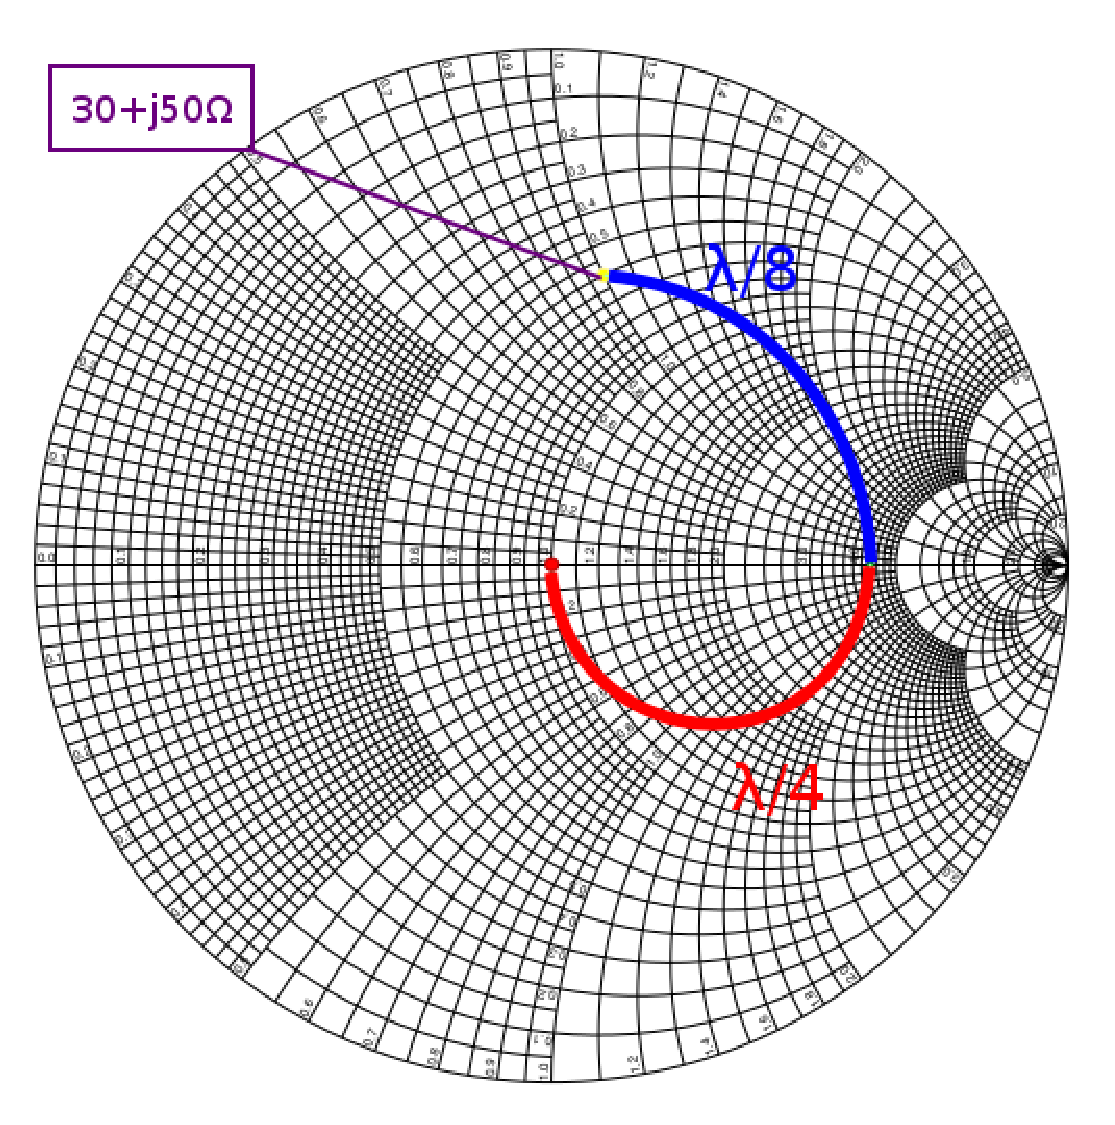
\includegraphics[width=120mm]{Smithl8l4}
\caption{Example of $\lambda/4 + \lambda/8$ matching: $Z_S = 50\Omega$, $Z_L = 30+j50\Omega$, $Z_{\lambda/4} = 102.6\Omega$, $Z_{\lambda/4} = 58.3\Omega$}
\label{fig:SmithL8L4}
\end{figure}


\noindent Design equations:
\begin{align}
Z_{\lambda/8} & = \sqrt{R_L^2 + X_L^2} \\
Z_{\lambda/4} & = \sqrt{\frac{R_S \cdot R_L \cdot Z_{\lambda/8}}{Z_{\lambda/8}-X_L}}
\end{align}


\noindent \textit{Reference:} \cite{BahlFundamentalsRFMW}, pages 159-161.


\subsection{Multistage $\lambda$/4 sections}
Typically, broadband matching between real impedances at microwave frequencies is done with multisection transformers. This matching technique relies on the \textit{Theory of the small reflections} which states that the overall reflection coefficient of N cascaded transmission lines of the same length can be approximated as:

\begin{equation}
\Gamma(\theta) = \sum \limits_{n=0}^{N} \Gamma_n \cdot e^{-j\cdot 2n \theta}
\label{eq:CascadeReflection}
\end{equation}

\noindent where $\theta$ is the electrical length of a single transmission line (typically $\lambda/4$). The ${\Gamma_n}$ weigths define the shape of $\Gamma(\theta)$ and they are taylored so as to get a binomial or a Chebyshev overall response.

\noindent Once given $\Gamma_n \;\; \forall n \in [0, N]$, it is possible to calculate the impedance of each transmission line:

\begin{equation}
Z_{n+1} \sim Z_n \cdot e^{2\cdot\Gamma_n}
\end{equation}

\noindent where n indicates the section number.

\subsubsection{Binomial weighting}
\noindent $\Gamma_n$ is defined as:

\begin{equation}
\Gamma_n = A\cdot C^{N}_{n} \;\; \forall n \in [0, N]
\end{equation}

\noindent where $A = 2^{-N}\frac{Z_L - Z_0}{Z_L + Z_0}$ and $C^N_n = \frac{N!}{(N-n)!n!}$

\subsubsection{Chebyshev weighting}

\noindent The overall reflection coeffient is set to:

\begin{equation}
\Gamma(\theta) = A \cdot e^{-jN\theta} \cdot T_{\theta}(sec(\theta_m)cos(\theta))
\end{equation}

\noindent where:

\begin{equation}
 A = \frac{Z_L - Z_0}{Z_L + Z_0} \cdot \frac{1}{T_N(sec(\theta_m))}
\end{equation}

\begin{equation}
  sec(\theta_m) = cosh(\frac{1}{N} acosh\left( \frac{1}{\Gamma_m} \lvert \frac{Z_L - Z_0}{Z_L + Z_0} \rvert \right))
\end{equation}

\noindent and $T_N(x)$ is the Chebyshev polynomial of order N. The Chebyshev polinomials are defined such that:
\begin{equation}
 T_n(x) = 2xT_{n-1}(x) - T_{n-1}(x)
\end{equation}

\begin{equation}
T_1(x) = x
\end{equation}

\begin{equation}
T_0(x) = 1
\end{equation}

\noindent $T_N(sec(\theta_m)cos(\theta))$ involves terms such as $cos^N(x)$, $cos^{N-1}(x)$,... In order to equate this terms to the $\Gamma_n$ terms in \ref{eq:CascadeReflection}, it is necessary to expand $cos^N(x)$ terms into sums of terms such as $cos((n-2m)\theta)$

\noindent \textit{Reference:} \cite{Pozar}, pages 250-260.

\subsection{Cascaded L-sections}
An alternative method to achieve broadband matching between real impedances is to cascade N (lowpass) \textit{L-section} stages. In this sense, the \textit{Cascaded L-sections} method does N-1 matches between intermediate real impedances such that $R_i > R_{i+1} \forall i \in N$.

\begin{figure}[H]
\centering
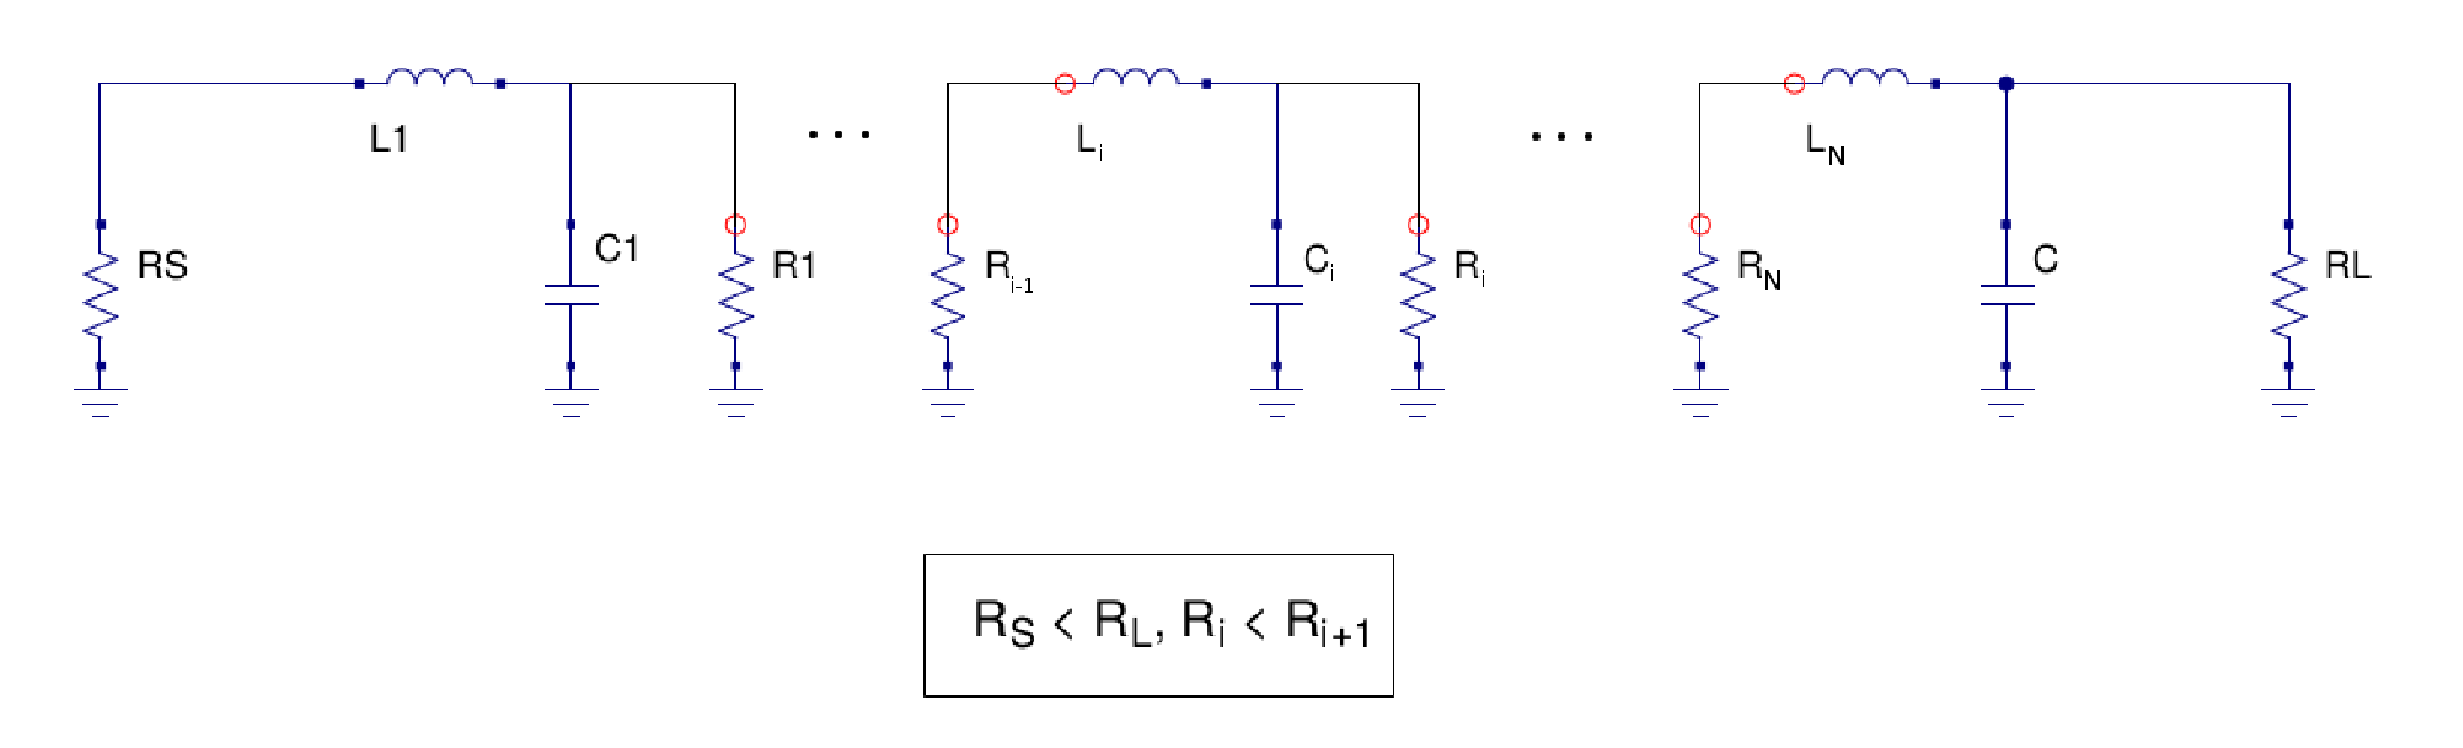
\includegraphics[width=120mm]{CascadedLCsch}
\caption{Cascaded L-sections method}
\end{figure}

Depending on the values of the intermediate impedances, the bandwidth of the matching network will vary. In order to maximize it, the ratios of consecutive virtual resistances should be equal:

\begin{equation}
  \frac{R_S}{R_1} = ... = \frac{R_{i}}{R_{i+1}} = ... = \frac{R_{N-1}}{R_{L}}
\end{equation}

\noindent Thus, the intermediate virtual resistance is given by:

\begin{equation}
R_i = R_S^{\frac{N-i}{N}} \cdot R_L^{\frac{i}{N}}, \forall i \in [1, N-1]
\end{equation}


\noindent Once having $R_i$, the values of the inductors and the can be determined:
\begin{align}
Q_i & = \sqrt {\frac{R_{i-1}}{R_i}},\\
C_i & = \frac{Q_i}{\omega R_{i-1}}, \\
L_i & = \frac{Q_i R_i}{\omega},  \forall i \in [1, N-1]
\end{align}


\begin{figure}[H]
\centering
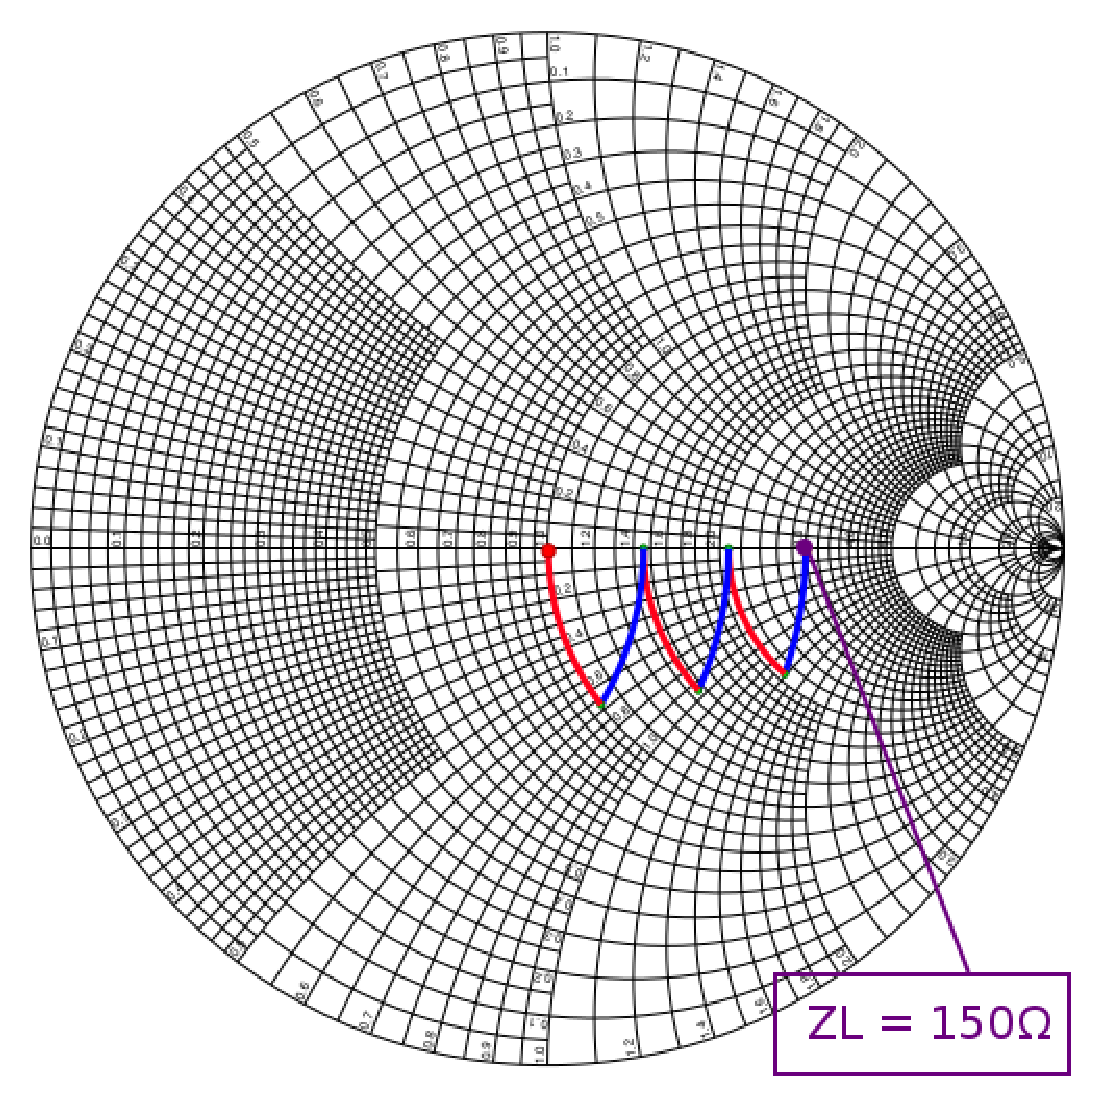
\includegraphics[width=120mm]{SmithCascadedLCsections}
\caption{Example of \textit{cascaded L-sections} matching: $Z_S = 50\Omega$, $Z_L = 150\Omega$, $L_i = \lbrace 5.3, 7.6, 11\rbrace nH$, $C_i = \lbrace 1.47, 1, 0.7 \rbrace pF$}
\end{figure}


\noindent \textit{Reference:} \cite{BahlFundamentalsRFMW}, pages: 169-172.
